%%%%%%%% ICML 2025 EXAMPLE LATEX SUBMISSION FILE %%%%%%%%%%%%%%%%%

\documentclass{article}

% Recommended, but optional, packages for figures and better typesetting:
\usepackage{microtype}
\usepackage{graphicx}
\usepackage{subfigure}
\usepackage{booktabs} % for professional tables

% hyperref makes hyperlinks in the resulting PDF.
% If your build breaks (sometimes temporarily if a hyperlink spans a page)
% please comment out the following usepackage line and replace
% \usepackage{icml2025} with \usepackage[nohyperref]{icml2025} above.
\usepackage{hyperref}


% Attempt to make hyperref and algorithmic work together better:
\newcommand{\theHalgorithm}{\arabic{algorithm}}

% Use the following line for the initial blind version submitted for review:
% \usepackage{icml2025}

% If accepted, instead use the following line for the camera-ready submission:
\usepackage[accepted]{icml2025}

% For theorems and such
\usepackage{amsmath}
\usepackage{amssymb}
\usepackage{mathtools}
\usepackage{amsthm}

% if you use cleveref..
\usepackage[capitalize,noabbrev]{cleveref}

% control list spacing
\usepackage{enumitem} % Recommended for better control over lists
\setlist[itemize]{itemsep=0em} % Globally set item spacing for itemize
\setlist[enumerate]{itemsep=0em} % Globally set item spacing for enumerate

%%%%%%%%%%%%%%%%%%%%%%%%%%%%%%%%
% THEOREMS
%%%%%%%%%%%%%%%%%%%%%%%%%%%%%%%%
\theoremstyle{plain}
\newtheorem{theorem}{Theorem}[section]
\newtheorem{proposition}[theorem]{Proposition}
\newtheorem{lemma}[theorem]{Lemma}
\newtheorem{corollary}[theorem]{Corollary}
\theoremstyle{definition}
\newtheorem{definition}[theorem]{Definition}
\newtheorem{assumption}[theorem]{Assumption}
\theoremstyle{remark}
\newtheorem{remark}[theorem]{Remark}

% Todonotes is useful during development; simply uncomment the next line
%    and comment out the line below the next line to turn off comments
%\usepackage[disable,textsize=tiny]{todonotes}
\usepackage[textsize=tiny]{todonotes}


% The \icmltitle you define below is probably too long as a header.
% Therefore, a short form for the running title is supplied here:
\icmltitlerunning{Delaunay Rewiring to Avoid Over-Squashing and Over-Smoothing in Graphs}

\begin{document}

\twocolumn[
\icmltitle{Delaunay Rewiring to Avoid Over-Squashing and Over-Smoothing in Graphs}

% It is OKAY to include author information, even for blind
% submissions: the style file will automatically remove it for you
% unless you've provided the [accepted] option to the icml2025
% package.

% List of affiliations: The first argument should be a (short)
% identifier you will use later to specify author affiliations
% Academic affiliations should list Department, University, City, Region, Country
% Industry affiliations should list Company, City, Region, Country

% You can specify symbols, otherwise they are numbered in order.
% Ideally, you should not use this facility. Affiliations will be numbered
% in order of appearance and this is the preferred way.
\icmlsetsymbol{equal}{*}

\begin{icmlauthorlist}
\icmlauthor{Edwin Roussin}{equal,ipp}
\icmlauthor{Tristan Waddington}{equal,ipp}

\end{icmlauthorlist}

\icmlaffiliation{ipp}{Institut Polytechnique de Paris, Palaiseau, France}

\icmlcorrespondingauthor{}{firstname.lastname@polytechnique.edu}

% You may provide any keywords that you
% find helpful for describing your paper; these are used to populate
% the "keywords" metadata in the PDF but will not be shown in the document
\icmlkeywords{Graph, Delaunay, Triangulation, Machine Learning, Over-smoothing, Over-squashing}

\vskip 0.3in
]

% this must go after the closing bracket ] following \twocolumn[ ...

% This command actually creates the footnote in the first column
% listing the affiliations and the copyright notice.
% The command takes one argument, which is text to display at the start of the footnote.
% The \icmlEqualContribution command is standard text for equal contribution.
% Remove it (just {}) if you do not need this facility.

% \printAffiliationsAndNotice{}  % leave blank if no need to mention equal contribution
\printAffiliationsAndNotice{\icmlEqualContribution} % otherwise use the standard text.

\begin{abstract}
This document reviews the graph rewiring method proposed by \cite{attali2024delaunay}
based on Delauynay triangulation that aims to avoid over-smoothing and over-squashing
during prediction tasks. It uses notions of edge curvature to measure the quality
of the rewiring. The method is tested on a variety of graph datasets and compared
to another one.
%TODO present other article
\end{abstract}

%%%%%%%%%%%%%%%%%%%%%%%%%%%%%%%%%%%%%%%%%%%%%%%%%%%%%%%%%%%%%%%%%%%%%%%%%%%%%%%
% Delaunay paper
%%%%%%%%%%%%%%%%%%%%%%%%%%%%%%%%%%%%%%%%%%%%%%%%%%%%%%%%%%%%%%%%%%%%%%%%%%%%%%%

\section{Delaunay Rewiring}
\label{delaunay}
Graph neural networks (GNNs) have emerged as the standard approach for effective
learning graph-structured data. GNNs employ an iterative approach, updating node repre-
sentations through the local aggregation of information from
neighboring nodes, known as the message-passing paradigm \cite{gilmer2017neural}.
However, this iterative process can lead to over-smoothing and over-squashing, where
the node representations become too similar to each other, or ineffective to 
transmit long-range information. In these cases, the model performance can degrade.

%%%%%%%%%%%%%%%%%%%%%%%%%%%%%%%%%%%%%%%%%%%%%%%%%%%%%%%%%%%%%%%%%%%%%%%%%%%%%%%
% Theoretical
\subsection{Over-Smoothing and Over-Squashing}

\paragraph{Over-Smoothing}
Message-passing neural networks (MPNN) use an 
iterative approach, updating node representations through 
the local aggregation of information from neighboring nodes.
The need to stack additional layers to capture non-local interactions
tends to make node features more and
more similar, leading to over-smoothing. This is particularly problematic 
when the graph is heterophilic, i.e., when nodes belong to different communities 
\cite{zheng2022graph}.

\paragraph{Over-Squashing}
The squashing effect occurs when the model is unable to transmit
long-range information, leading to a loss of information. MPNN models try to 
capture exponentially growing information into fixed sized representations. 
\cite{alon2021bottleneck} have shown the correlation between overs-quashing and 
 bottleneck in the graph structure.
Models such as Graph Convolutional Networks (GCN) are known to suffer from this issue
because they absorb  the information from all edges equally.

%%%%%%%%%%%%%%%%%%%%%%%%%%%%%%%%%%%%%%%%%%%%%%%%%%%%%%%%%%%%%%%%%%%%%%%%%%%%%%%
\subsection{Edge Curvature}
The main metrics used to characterize graph structure and measure the quality
of the rewiring is the discrete Ricci edge curvature. A complete definition can be found on 
\cref{app:curvature}. Previous work has shown that:
\begin{itemize}
    \item Positive curvature edges establish connections between 
        nodes belonging to the same community.
        Highly positive curved edges cause over-smoothing \cite{nguyen2023revisiting}.
                
    \item Negative curvature edges connect nodes from different communities.
        Highly negative curved edges cause over-squashing \cite{topping2022understandingoversquashingbottlenecksgraphs}.
\end{itemize}
\begin{figure}[ht]

    \vskip -0.2in
    \begin{center}
    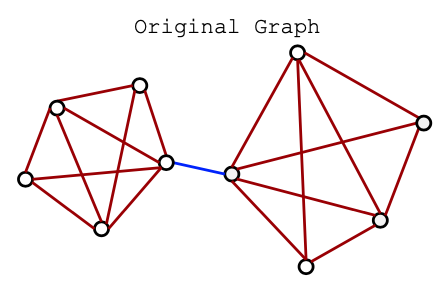
\includegraphics[width=0.6\columnwidth]{figures/original_graph.png}
    \caption{\scriptsize Example graph: in red the edges with positive curvature ($\sim 3$), 
    in blue with negative curvature (-1.2) \cite{attali2024delaunay}}
    \label{fig:edge_curvature}
    \end{center}
    \vskip -0.2in
\end{figure}
\textbf{Hence, we get a simple metric for further experiments where we expect to see the 
edge curvature amplitude decrease after the rewiring process.}

%%%%%%%%%%%%%%%%%%%%%%%%%%%%%%%%%%%%%%%%%%%%%%%%%%%%%%%%%%%%%%%%%%%%%%%%%%%%%%%
\subsection{Rewiring}
\subsubsection{Former methods' limitation}
Existing methods mitigate over-squashing by rewiring
the input graph to minimize structural bottlenecks. 
First ones rely on the analysis of the graph structure, through local or global features
like edge curvature or resistance. However, these methods may not scale well with 
the number of nodes and need depends on the choice of hyperparameters. 
Moreover, they modify the original graph, which is not always available in some applications.

Conversely, over-smoothing is avoided by preventing embedding to become the same 
through: \textbf{Normalization} with PairNorm \cite{zhao2020pairnorm}; 
or \textbf{rewiring} dropping edges, at random \cite{rong2019dropedge} 
or in finding the potential good ones \cite{Giraldo_2023}

\subsubsection{Delaunay Triangulation}
\paragraph{Delaunay rewiring}
Is an extreme \textbf{4 steps rewiring} method illustrated bellow and detailed 
in \cref{alg:delaunay}:
\begin{enumerate}
    \item A first GNN\footnote{GCN from \cite{kipf2017semi}} constructs 
        \textbf{node embeddings} from the original graph.
    \item Reduce the embedding with \textbf{UMAP} in dim 2.
    \item \textbf{Rebuild edges with Delaunay triangulation} from their distance in UMAP embedding space.
    \item Second GNN \textbf{mix} the Delaunay graph with the original features 
    from the beginning.
\end{enumerate}
\begin{figure}[ht!]
    \begin{center}
    \vskip -0.2in
    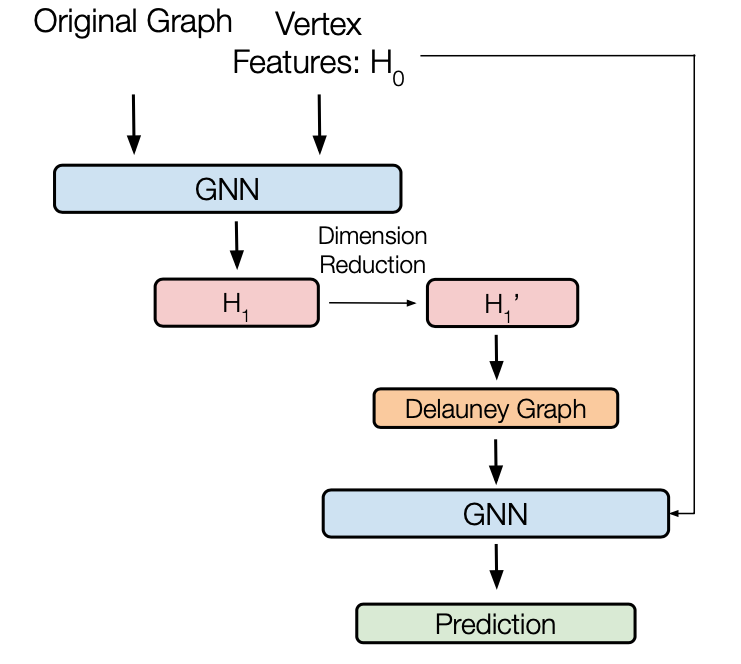
\includegraphics[width=0.8\columnwidth]{figures/Rewiring_method_s.png}
    \caption{Illustration of the Delaunay [Attali al., 2024] \cite{attali2024delaunay}}
    \vskip -0.2in
    \label{fig:delaunay_rewiring}
    
    \end{center}
\end{figure}

\begin{algorithm}[htb!]
    \caption{Delaunay Rewiring}
    \label{alg:delaunay}
 \begin{algorithmic}
    \STATE {\bfseries Input:} dataset $x$, graph $G = (H_0, E)$
    \STATE Compute node embeddings $H_1$ with GNN1 from $G$ \COMMENT{if needed}
    \STATE Reduce  to 2D with UMAP $H_1 \to H_2$
    \STATE Compute Delaunay triangulation $DT(H_2)$
    \STATE $E' = \emptyset$
    \FOR{$(i, j) \in DT(H_2).simplices$}
        \STATE $E' = E' \cup \{(i, j)\}$  \COMMENT{Add undirected edge}
    \ENDFOR
    \STATE  $G' = (H_2, E')$  \COMMENT{Rewired graph}
    \STATE Compute node embeddings $H'$ with GNN2 from $G'' = (H_0, H_2, E')$
    {\bfseries Return:}  predicted class of nodes
 \end{algorithmic}
 \end{algorithm}

\paragraph{GNN embedding}
Initially, the authors triangulated the graphs considering the original 
features. However, these starting features often lack
expressiveness or suffer from poor quality. So they used the strategy to pass
add the first step of GNN embedding to improve the quality of the Delaunay graph.
In our following experiment, the intial embedding is not used as the data 
is good enough. We did not experiment this part.





\paragraph{Initial thoughts}
The method is remarkably simple, as it does not require any hyperparameters according to authors, 
which eliminates the need for a grid search. Its computational complexity is 
efficient, scaling as $\mathcal{O} \big( N \log N \big)$. 
Additionally, the method constructs a graph directly from the embedding, 
making it independent of the presence of the original graph.

The use of UMAP is restricted to two dimensions. This is because performing 
triangulation in higher dimensions increases computation time and 
results in denser graphs\footnote{Generalized triangles in three dimensions
 have six edges, while in four dimensions, they have ten edges.}. 
This increased density reduced the accuracy in experiments, making the two-dimensional approach more practical and effective.

Authors have added the first GNN late in their research as the Delaunay Graph 
need quality embedding. However, it raises questions about whether these initial
representation are victims of smoothing and squashing effects by this GNN.
Does this GNN effectively captures long-range dependencies?


%%%%%%%%%%%%%%%%%%%%%%%%%%%%%%%%%%%%%%%%%%%%%%%%%%%%%%%%%%%%%%%%%%%%%%%%%%%%%%%
\subsection{Experiments}
We have reproduced the rewiring experiment on the \textbf{Wisconsin dataset}\footnote{
From WebKB dataset, 251 nodes = web pages from Wisconsin connected
by edges = hyperlinks, node features = bag-of-words in dim 1703, labels =  5 kind of author.}.
The report in \cref{tab:metric_comparison} demonstrate substantial improvements in graph neural network performance. The effect
of the Delaunay rewiring is clearly visible on the degree distribution in the \cref{fig:degree_dist} below.
The curvature distribution of the edges is also shown in the \cref{fig:delaunay_curvature}.

\textbf{Key Results}:
    GCN accuracy improved from $54.90\%$ to $67.55\%$ $(+12.6\%)$.
    GAT accuracy improved from $55.88\%$ to $69.12\%$ $(+13.2\%)$.
    Graph homophily increased by $96\%$ ($0.366 \to  0.718$).
    All improvements are statistically significant ($p<0.0001$).

\begin{figure}[ht]
    \begin{tabular}{cc}
        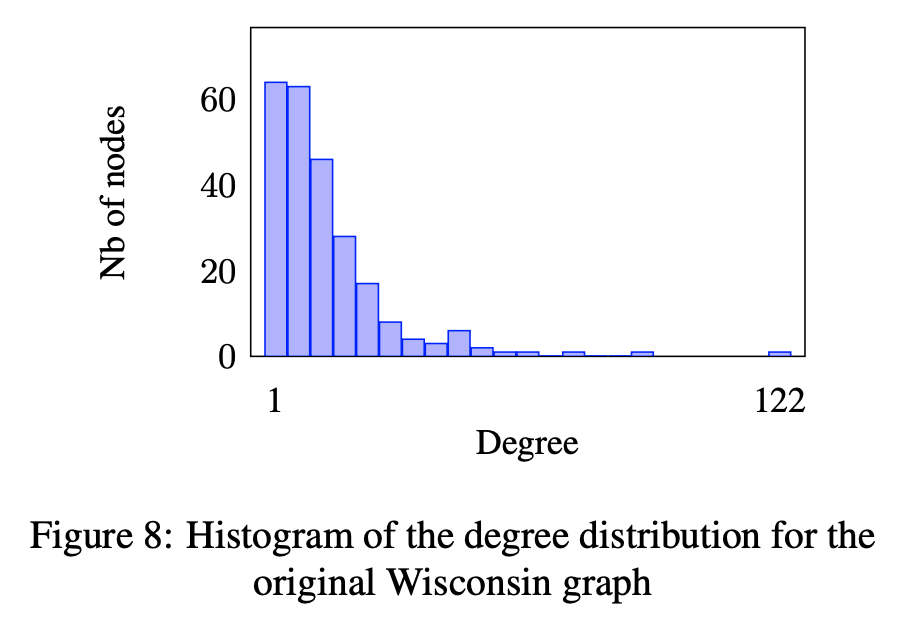
\includegraphics[width=0.4\columnwidth]{figures/Wisconsin_degree_distrib_original.png} &
        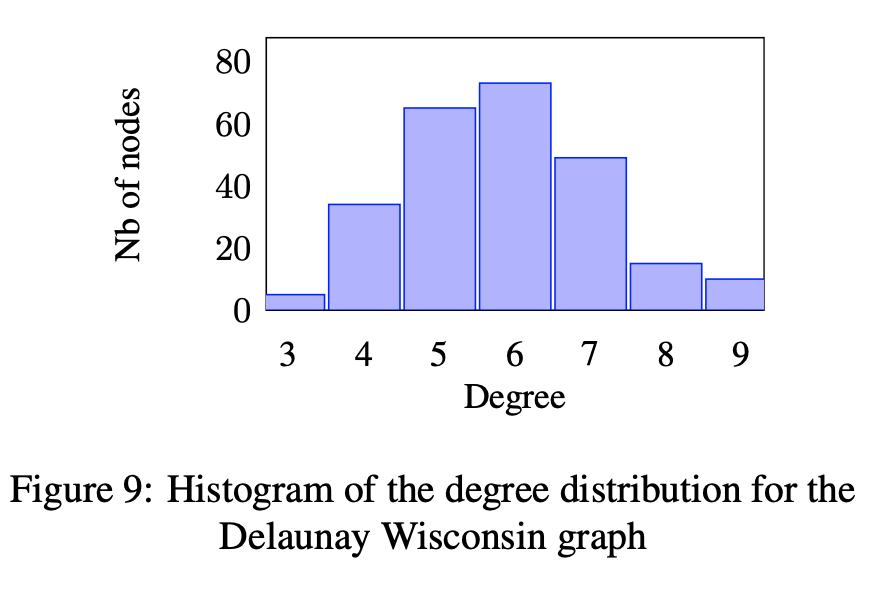
\includegraphics[width=0.4\columnwidth]{figures/Wisconsin_degree_hist_original.png} \\
        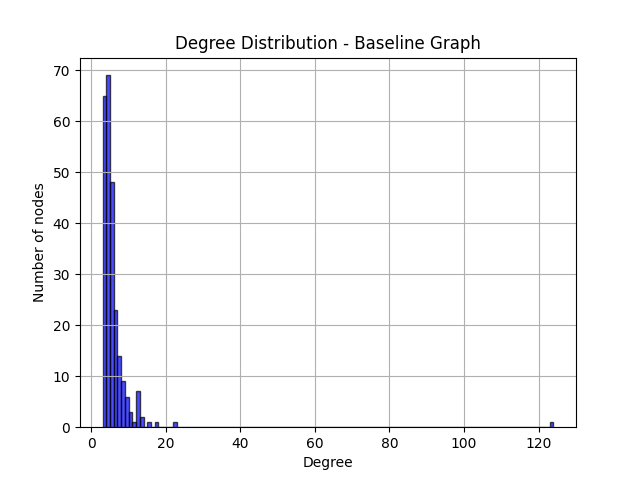
\includegraphics[width=0.4\columnwidth]{figures/baseline_degree_dist_baseline_graph_20250314_180715.png} &
        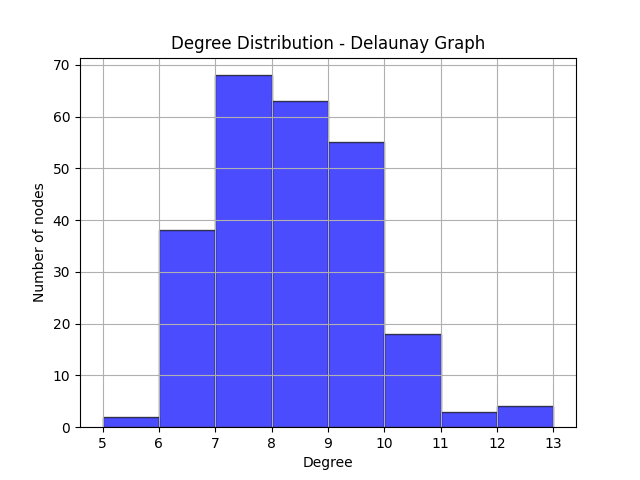
\includegraphics[width=0.4\columnwidth]{figures/delaunay_degree_dist_delaunay_graph_20250314_180840.png}
    \end{tabular}
    \vskip -0.2in
    \caption{Effect of the Delaunay rewiring on degree distribution. 
                Left: original, Right: after rewiring, Top: [Attali al., 2024] \cite{attali2024delaunay}, Bottom: ours.}
    \label{fig:degree_dist}
\end{figure}


\begin{table}[b]
    \caption{Comparison of Baseline and Delaunay Graph Metrics}
    \centering
    \begin{tabular}{|l|c|c|}
        \hline
        \textbf{Metric}          & \textbf{Orignal} & \textbf{Delaunay Graph} \\ \hline
        Mean Degree              & 5.59                   & 7.85               \\ \hline
        Homophily                & 0.366                  & 0.710 ($\uparrow$ 96\%) \\ \hline
        Curvature Range          & [-0.475, 0.250]        & [-0.214, 0.200]         \\ \hline
    \end{tabular}
    \label{tab:metric_comparison}
\end{table}
    
\textbf{Impact}: The Delaunay rewiring approach successfully addresses 
over-squashing and improves graph structure, leading to significant performance 
gains across different model architectures.

\begin{figure}[htb]
    \begin{center}
        \begin{tabular}{cc}
            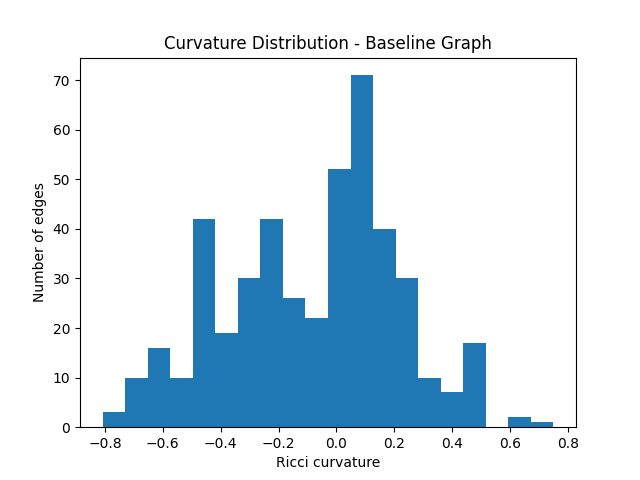
\includegraphics[width=0.4\columnwidth]{figures/baseline_curvature_dist_baseline_graph_20250321_203836.png}&
            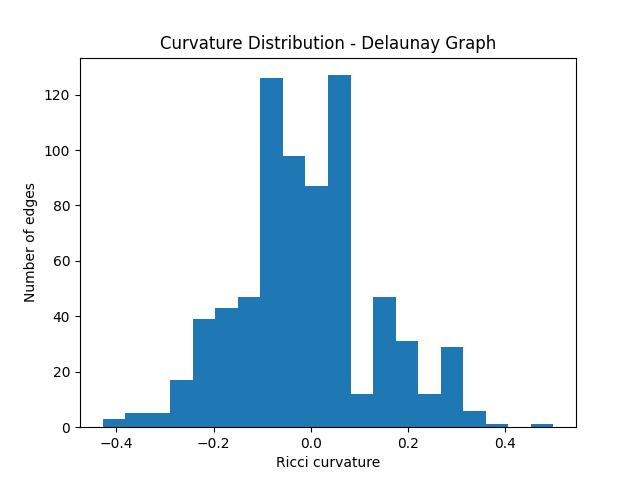
\includegraphics[width=0.4\columnwidth]{figures/delaunay_curvature_dist_delaunay_graph_20250321_204407.png}
        \end{tabular}
    \vskip -0.2in
    \caption{Evolution of the curvature distribution of nodes after rewiring (right).
    We can confirm that the amplitude of the curvature has decreased.}
    \label{fig:delaunay_curvature}
    \end{center}
\end{figure}

\textbf{Validation}: Results are robust across multiple experiments and 
statistically significant, with comprehensive analysis of graph properties
supporting the improvements.

%%%%%%%%%%%%%%%%%%%%%%%%%%%%%%%%%%%%%%%%%%%%%%%%%%%%%%%%%%%%%%%%%%%%%%%%%%%%%%%
\subsection{Limitations}
\paragraph{Dimensionality Reduction} We might lose some feature information
during the UMAP reduction to 2 dimensions. The quality of Delaunay graph depends
 on quality of reduced features.

 \paragraph{Computational Considerations}
 The method complexity is in $\mathcal{O} \big( N \log N \big)$ only, but the 
 two graphs are  fully loaded into memory. Furthermore, the UMAP and curvature 
 computation can cause overhead, but this is way better than the quadratic cost
 of other methods.
   
\paragraph{Parameter Sensitivity} We do not entirely agree with the authors as
we find out that the impact of UMAP parameters not fully explored. They could
modulate the quality of the embedding we already discussed. Moreover, the
potential dependence on feature normalization and the effect of different
 train/val/test splits is not extensively studied.

\subsection{Future Work}
If we were to work further in this topic, we could focus on:
\begin{itemize}
    \item \textbf{Algorithmic Improvements}: Investigate higher-dimensional 
    Delaunay triangulation, explore sparse approximations for larger graphs, 
   Develop incremental/streaming versions for large-scale graphs or 
   optimize UMAP parameter selection.

    \item \textbf{Analysis Extensions}:
   Study impact on different graph properties, 
   investigate relationship between feature space and graph structure,
   compare with other rewiring methods on the same dataset,
   or analyze feature importance in graph construction.

    \item \textbf{Ablation Studies}:
   Compare with other dimensionality reduction method, the effect of different 
   feature preprocessing, the sensitivity to hyperparameters and try different
    triangulation algorithms.
\end{itemize}

%%%%%%%%%%%%%%%%%%%%%%%%%%%%%%%%%%%%%%%%%%%%%%%%%%%%%%%%%%%%%%%%%%%%%%%%%%%%%%%
% Other paper
%%%%%%%%%%%%%%%%%%%%%%%%%%%%%%%%%%%%%%%%%%%%%%%%%%%%%%%%%%%%%%%%%%%%%%%%%%%%%%%
\section{Additional Paper}
We have chosen to delve into another rewiring method proposed by \cite{wilson2024cayleygraphpropagation}
based on Cayley graphs, named \textbf{Cayley Graph Propagation}. 
The authors have focus on the creation of bottleneck-free
structure to ameliorate the over-squashing effect. 

% TODO
%%%%%%%%%%%%%%%%%%%%%%%%%%%%%%%%%%%%%%%%%%%%%%%%%%%%%%%%%%%%%%%%%%%%%%%%%%%%%%%
\subsection{Choice explanation}
We selected this paper because it aligns with the concept of \textbf{rewiring
the initial graph using a mathematical structure}.
On one hand, Delaunay Triangulation leverages geometric properties. 
On the other hand, the Cayley graph is a mathematical structure that can represent a group.
We believe these two methods are both competitive and complementary.
Notably, both papers were published in 2024 and do not reference each other.

%%%%%%%%%%%%%%%%%%%%%%%%%%%%%%%%%%%%%%%%%%%%%%%%%%%%%%%%%%%%%%%%%%%%%%%%%%%%%%%
\subsection{Paper summary}
\cite{wilson2024cayleygraphpropagation} focuses on the over-squashing effect.
Their aim is to \textbf{precompute bottleneck-free graph structures} to alleviate the
over-squashing effect. They propose the use of a well-known \textbf{expander graph} family:
the Cayley graphs of the $\text{SL}(2,\mathbb{Z}_n)$ special linear group as a computational template for GNNs.

They have improved previous work already used this family that required to 
truncate the graph to align with the input graph. The authors show that truncation is
not necessary and that the complete Cayley graph can be used directly with 
the direct effect of reducing the diameter of the graph as illustrated in the \cref{fig:cayley_graph}.


\begin{figure}[htb!]
    \begin{center}
        \begin{tabular}{cc}
            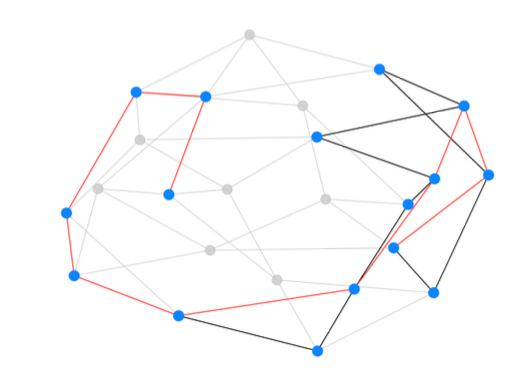
\includegraphics[width=0.4\columnwidth]{figures/Cayley1.png}&
            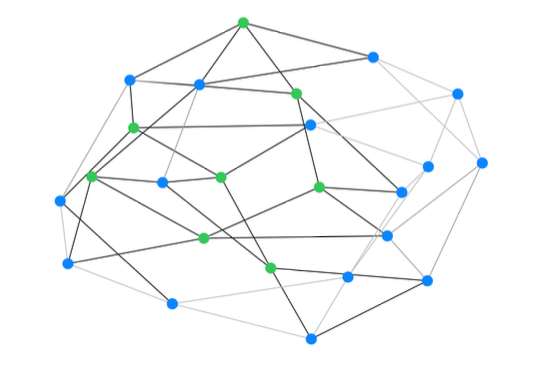
\includegraphics[width=0.4\columnwidth]{figures/Cayley2.png}
        \end{tabular}
    \vskip -0.2in
    \caption{Both Cayley graphs represent $SL(2,\mathbb{Z}_3)$ with $|V|= 24$ nodes using the same construction.
    Left: A truncated Cayley graph (spectral gap: $0.0751$, diameter: $10$) aligned to a given input graph.
    Right: The complete Cayley graph (spectral gap: $1.2679$, diameter: $4$) structure indicating the
    additional virtual nodes (in green). Source: \cite{wilson2024cayleygraphpropagation}}
    \label{fig:cayley_graph}
    \end{center}
\end{figure}

The authors have shown that the spectral gap of the Cayley graph is a good indicator
of the quality of the graph structure. A larger spectral
gap defines a strong connectivity, or alternatively the global lack of bottlenecks.
The spectral gap is the difference between the first and second normalized eigenvalues of the graph Laplacian.

%%%%%%%%%%%%%%%%%%%%%%%%%%%%%%%%%%%%%%%%%%%%%%%%%%%%%%%%%%%%%%%%%%%%%%%%%%%%%%%
\subsection{Comparison}


The constructed Cayley graph with $|V|$ nodes has a low diameter, requiring only
$\mathcal{O}(log(|V(G)|)$ steps to globally propagate information. This enhances
its ability to eliminate over-squashing and bottlenecks, which is further 
supported by having a higher spectral gap.

But this construction requires to add new nodes into the graph; hence, we need to modify the feature
matrix into an extended version, $\mathbf{X}' \in \mathbb{R}^{(|V| + virt)| \times d}$.
The first $|V|$ nodes are featured using the data from $\mathbf{X}$, the vitrual 
ones are initialized as zeros.


Furthermore, this new method does not suffer from limitations of the Cayley graph construction:
the inability to find the best way to align it to a given input graph, mitigating the potential for
stochastic effects in the process. The additional virtual nodes act as “bridges” between poorly
connected communities in the Cayley graph, ameliorating any poorly-connected regions caused by
misalignment: see how the former red string in now connected in the \cref{fig:cayley_graph}.
However, the absence of curvature metrics in the Cayley graph makes it difficult to compare the two methods
on the over-smoothing factor.


To compare these methods, we evaluated both approaches on the MUTAG dataset, 
a binary graph classification task containing $188$ molecular graphs. Using 
a $4$-layer GIN architecture with batch normalization and $5$-fold stratified 
cross-validation, we assessed each method's ability to preserve and leverage molecular 
graph structure. While CGP achieved strong performance ($92.01\% \pm 3.80\%$), 
Delaunay rewiring showed lower accuracy ($88.31\% \pm 2.64\%$), likely due to 
information loss during the dimensional reduction step. This suggests that preserving 
graph topology through virtual nodes, as in CGP, might be more effective than 
complete geometric rewiring for molecular property prediction tasks.


%%%%%%%%%%%%%%%%%%%%%%%%%%%%%%%%%%%%%%%%%%%%%%%%%%%%%%%%%%%%%%%%%%%%%%%%%%%%%%%
% Template conclusion
%%%%%%%%%%%%%%%%%%%%%%%%%%%%%%%%%%%%%%%%%%%%%%%%%%%%%%%%%%%%%%%%%%%%%%%%%%%%%%%

\section*{Software and Data}

The original code repository and additional work can be found on GitHub\footnote{ 
\url{https://github.com/waddason/Delaunay-Rewiring}}.
The code is written in Python and uses the PyTorch library. The code is available under the MIT license.

% Acknowledgements should only appear in the accepted version.
\section*{Acknowledgements}

We thank our professor Mr. Jhony H. Giraldo for presenting us this article and 
the theoretical foundations to understand it.

\section*{Impact Statement}

This paper highlight the promising yet simple method of Delauynay Rewirin to 
improve the performance of graph-based machine learning models.
We hope to see this method adopted.


% In the unusual situation where you want a paper to appear in the
% references without citing it in the main text, use \nocite
% \nocite{langley00}

\bibliography{references}
\bibliographystyle{icml2025}


%%%%%%%%%%%%%%%%%%%%%%%%%%%%%%%%%%%%%%%%%%%%%%%%%%%%%%%%%%%%%%%%%%%%%%%%%%%%%%%
%%%%%%%%%%%%%%%%%%%%%%%%%%%%%%%%%%%%%%%%%%%%%%%%%%%%%%%%%%%%%%%%%%%%%%%%%%%%%%%
% APPENDIX
%%%%%%%%%%%%%%%%%%%%%%%%%%%%%%%%%%%%%%%%%%%%%%%%%%%%%%%%%%%%%%%%%%%%%%%%%%%%%%%
%%%%%%%%%%%%%%%%%%%%%%%%%%%%%%%%%%%%%%%%%%%%%%%%%%%%%%%%%%%%%%%%%%%%%%%%%%%%%%%
\newpage
\appendix
\onecolumn

%%%%%%%%%%%%%%%%%%%%%%%%%%%%%%%%%%%%%%%%%%%%%%%%%%%%%%%%%%%%%%%%%%%%%%%%%%%%%%%
% Delaunay
%%%%%%%%%%%%%%%%%%%%%%%%%%%%%%%%%%%%%%%%%%%%%%%%%%%%%%%%%%%%%%%%%%%%%%%%%%%%%%%

\section{Additional details on the Delaunay Rewiring method}
\subsection{Delaunay Triangulation}
The Delaunay triangulation is a method to construct a graph from a set of points in a space.
It is a well-known method in computational geometry and has been used in various applications.

\label{app:delaunay}
\begin{figure}[h!]
    \center

    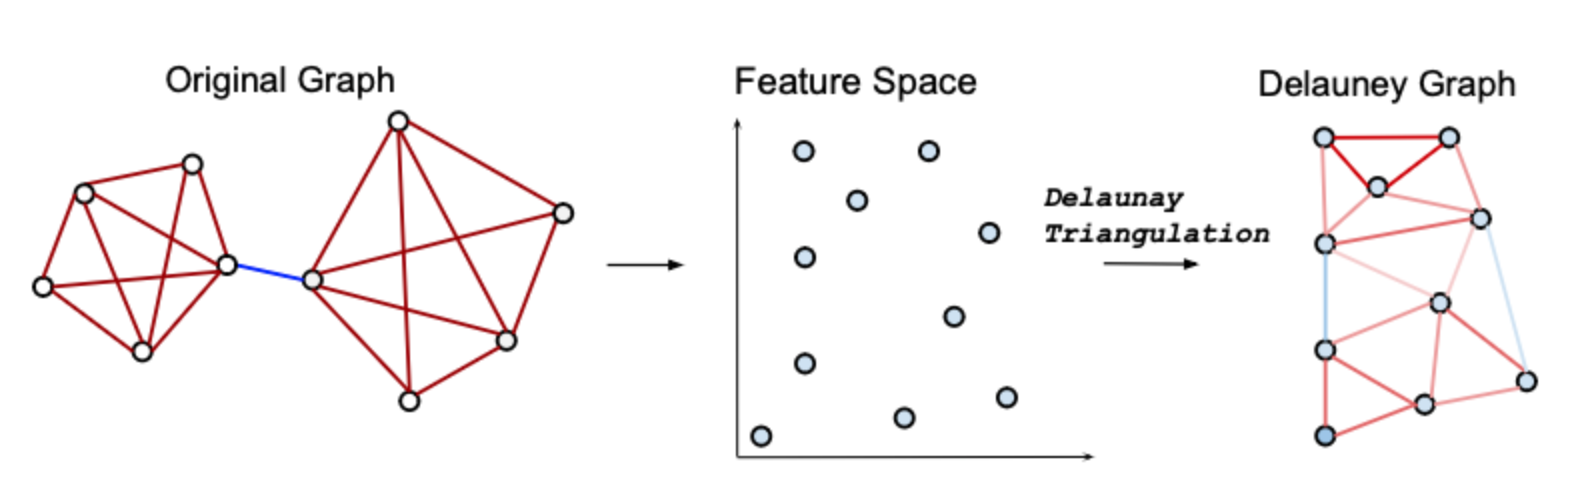
\includegraphics[width=0.9\textwidth]{figures/delaunay_process.png}
    \caption{Illustration of the Delaunay rewiring process in a 2-dimension feature space.}
    \label{fig:delaunay_full}
\end{figure}
\begin{definition}
    \label{def:delaunay}
A Delaunay triangulation, denoted as $DT(P)$, for a set $P$ of points 
        in the $d$-dimensional Euclidean space, is a triangulation where no 
        point in $P$ resides within the circum-hypersphere of any $d$-simplex 
        in $DT(P)$.
    \end{definition}

%%%%%%%%%%%%%%%%%%%%%%%%%%%%%%%%%%%%%%%%%%%%%%%%%%%%%%%%%%%%%%%%%%%%%%%%%%%%%%%
% Edge curvature

\subsection{Edge Curvature}
\label{app:curvature}
We describe bellow the two main curvature metrics used in the Delaunay rewiring method.
\paragraph{Paper}: 
Balance Forman Curvature \cite{topping2022understandingoversquashingbottlenecksgraphs} 
is computed over cycles of size 4.
    
\textbf{Balance Forman Curvature}:
    $$c_{ij}= \frac{2}{d_i} + \frac{2}{d_j} - 2 + 2 \frac{\sharp_{\Delta}}{\max(d_i, d_j)} + 
            \frac{\sharp_{\Delta}}{\min(d_i, d_j)} + 
            \frac{\max(\sharp_{\square}^i,\sharp_{\square}^j)^{-1}}{\max(d_i, d_j)}
            (\sharp_{\square}^i + \sharp_{\square}^j)
    $$

    where $\sharp_{\Delta}$ is the number of triangles based at $e_{ij}$, 
    $\sharp_{\square}^i$ is the number of 4-cycles based at $e_{ij}$ starting from $i$
    without diagonals inside.


\paragraph{Experiment}: 
\textbf{Oliver-Ricci Curvature} \cite{ni2015riccicurvatureinternettopology} 

We used the specific implementation from \texttt{GraphRicciCurvature.OllivierRicci}. 
Node Ricci curvature is defined as the average of all it’s adjacency edge. A visual
representation of the curvature of edges in a graph is shown in the \ref{fig:ricci_edge_curvature} below 
from the original paper.
\begin{figure}[ht!]
    \center
    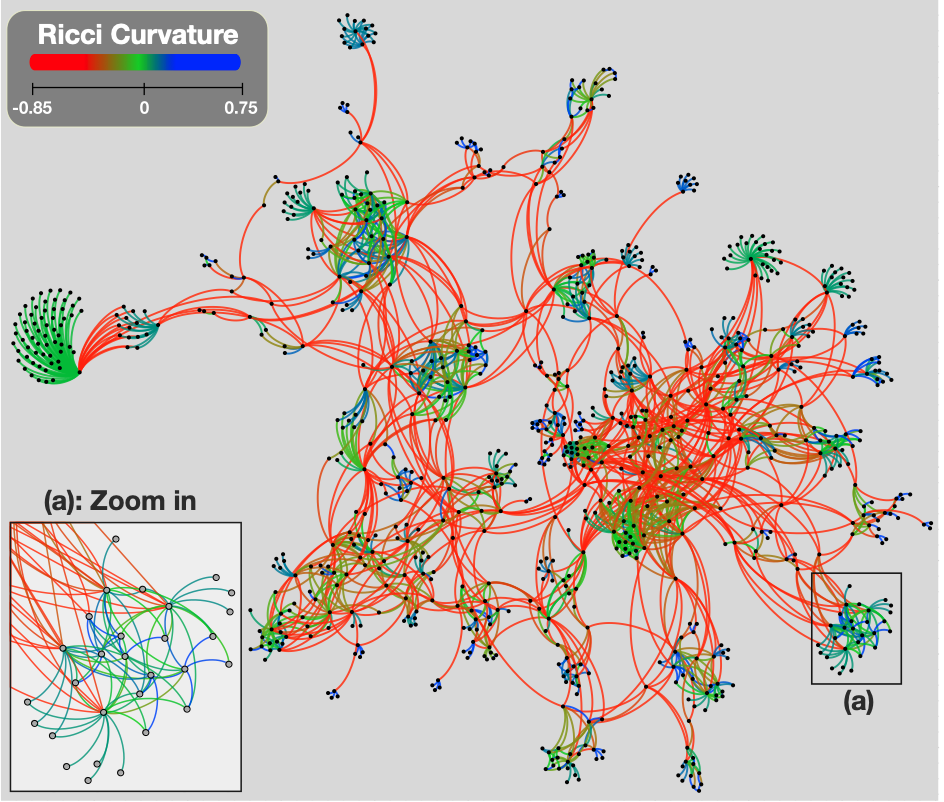
\includegraphics[width=0.6\textwidth]{figures/Riccicurvature.png}
    \caption{ It shows the Ricci curvature of each edge in a router level graph
    (Exodus(US)) from the Rocketfuel data set with 895 nodes and 2071
    edges. Negatively curved edges (in red) behave like “backbones”,
    maintaining the connectivity of clusters that are grouped by zero and
    positively curved edges (in green and blue). Source \cite{ni2015riccicurvatureinternettopology}}
    \label{fig:ricci_edge_curvature}
\end{figure}

%%%%%%%%%%%%%%%%%%%%%%%%%%%%%%%%%%%%%%%%%%%%%%%%%%%%%%%%%%%%%%%%%%%%%%%%%%%%%%%
% UMAP
\subsection{UMAP}
\paragraph{Method presentation}
Uniform Manifold Approximation and Projection (UMAP) is a dimensionality 
reduction technique that can be used for visualisation similarly to t-SNE,
but also for general non-linear dimension reduction.
UMAP constructs a high dimensional graph representation of the data 
then optimizes a low-dimensional graph to be as structurally similar as possible.

\begin{itemize}
    \item \textbf{Speed}: UMAP is faster than t-SNE.
    \item \textbf{Global structure}: UMAP preserves more of the global structure.
    \item \textbf{Separation}: clearly separate groups of similar categories.
\end{itemize}
Dimensionality reduction technique is not perfect - by necessity, we're distorting
 the data to fit it into lower dimensions - and UMAP is no exception. 
 But it is a powerful tool to visualize and understand large, high-dimensional datasets.

\paragraph{Hyperparameters choice}
Most common: \texttt{n\_neighbors} and \texttt{min\_dist}, control the balance between local and global structure.
They have a significant impact on the resulting embedding, and the choice of these parameters is crucial.
A visual example of their effect on the same two linked circles is shown in the \cref{fig:umap_hyperparam} below.
\begin{itemize}
    \item \texttt{n\_neighbors}: number of neighbors used to construct the high-dimensional graph.
    \item \texttt{min\_dist}: minimum distance between points in the low-dimensional space.
\end{itemize}
\begin{figure}[ht!]
    \center
    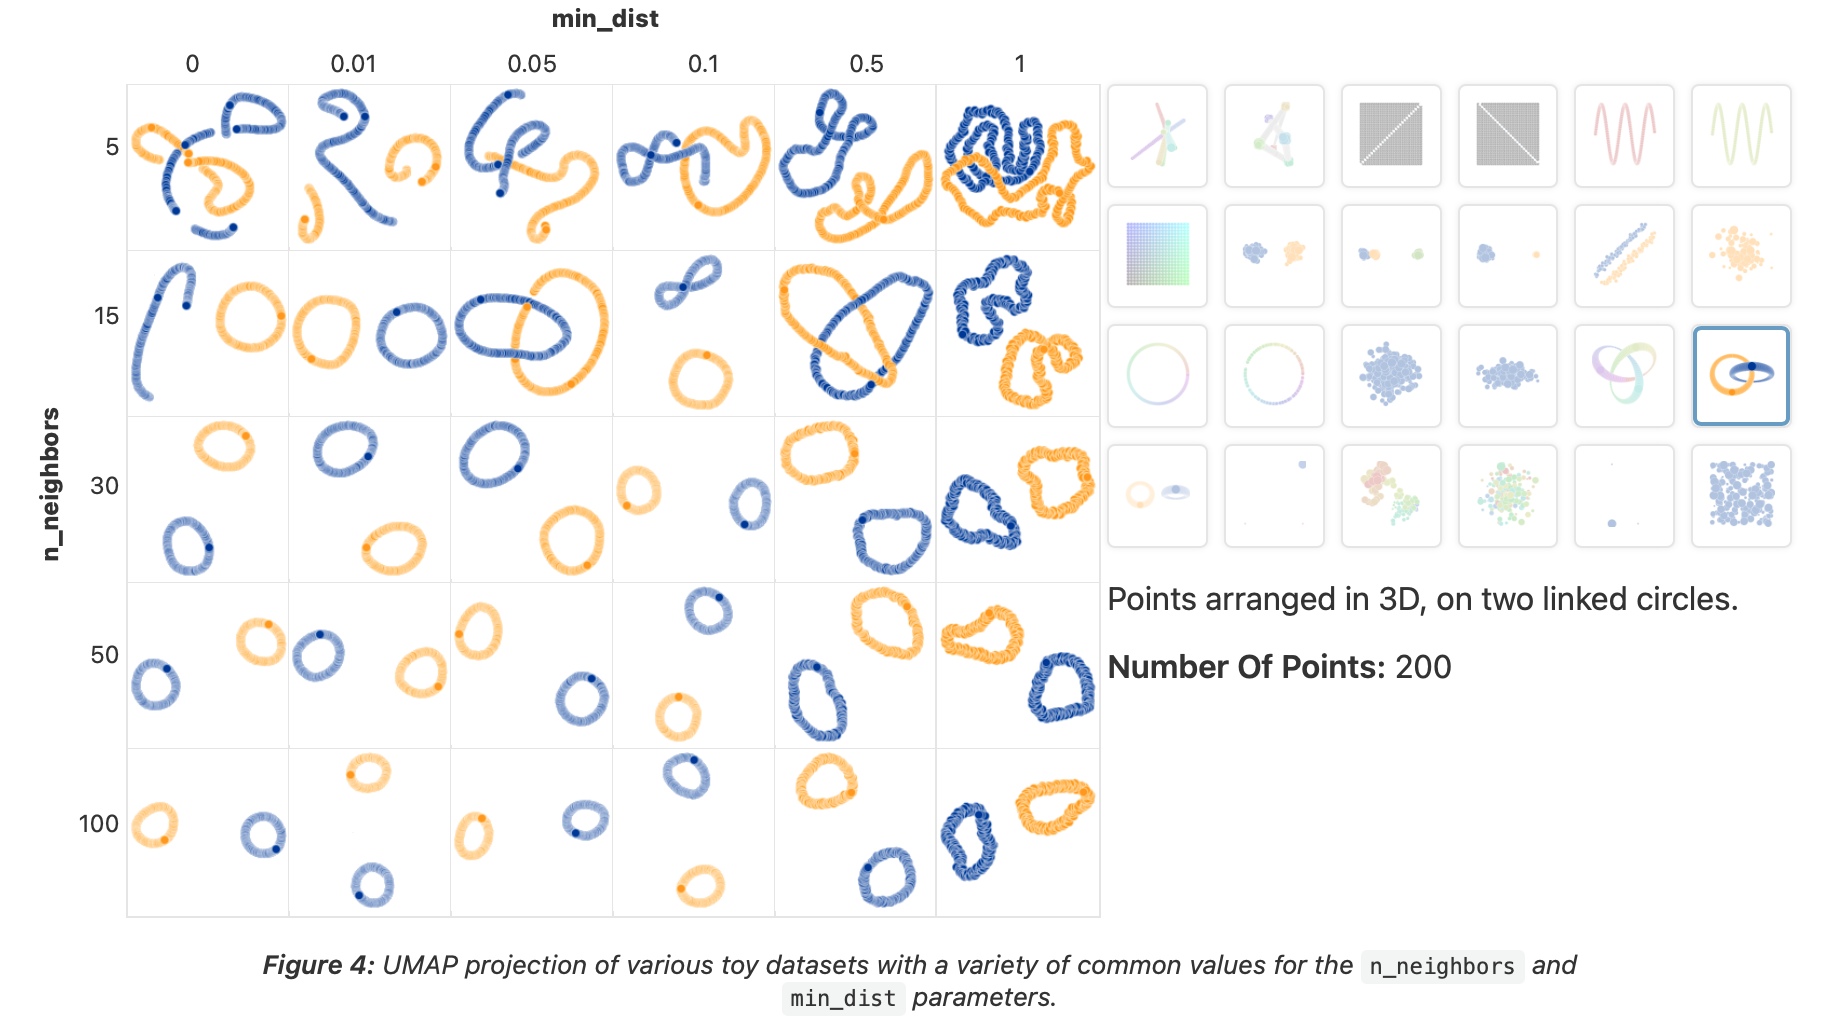
\includegraphics[width=0.8\textwidth]{figures/UMAP_hyperparam.png}
    \caption{\scriptsize Illustration of UMAP hyperparameters from 
        \href{https://pair-code.github.io/understanding-umap/index.html}{Google PAIR}}
    \label{fig:umap_hyperparam}
\end{figure}

%%%%%%%%%%%%%%%%%%%%%%%%%%%%%%%%%%%%%%%%%%%%%%%%%%%%%%%%%%%%%%%%%%%%%%%%%%%%%%%
% Experiment
%%%%%%%%%%%%%%%%%%%%%%%%%%%%%%%%%%%%%%%%%%%%%%%%%%%%%%%%%%%%%%%%%%%%%%%%%%%%%%%
\section{Experiment Details on the Delaunay Rewiring method}
%%%%%%%%%%%%%%%%%%%%%%%%%%%%%%%%%%%%%%%%%%%%%%%%%%%%%%%%%%%%%%%%%%%%%%%%%%%%%%%
\subsection{Wisconsin Dataset}
WebKB is a dataset that includes web pages from computer science departments of 
various universities. It represents $4,518$ web pages that are categorized into 6 imbalanced categories 
(Student, Faculty, Staff, Department, Course, Project). Additionally there is 
Other miscellanea category that is not comparable to the rest. We have used the
Wisconsin subset of the dataset, which contains 251 web pages from the University of Wisconsin-Madison.

We used the classical dataset splitting from Train/Val/Test Split: $60\%/20\%/20\%$ 
as proposed by \cite{attali2024delaunay}. We add our own data preprocessing in normalizaing the features.
Our experiment modestly reaches a $69.12\%$ accuracy on the Wisconsin dataset,
which has been outperformed by other methods since 2019 has shown in the leaderboard bellow.
\footnote{Highest accuracy on the Wisconsin dataset is $90.5\%$ by \cite{huang2024higherordergraphconvolutionalnetwork}, using
Higher-order Graph Convolutional Network (HiGCN) grounded in Flower Petals Laplacians, 
capable of discerning intrinsic features across varying topological scales. }

\begin{figure}[htb!]
    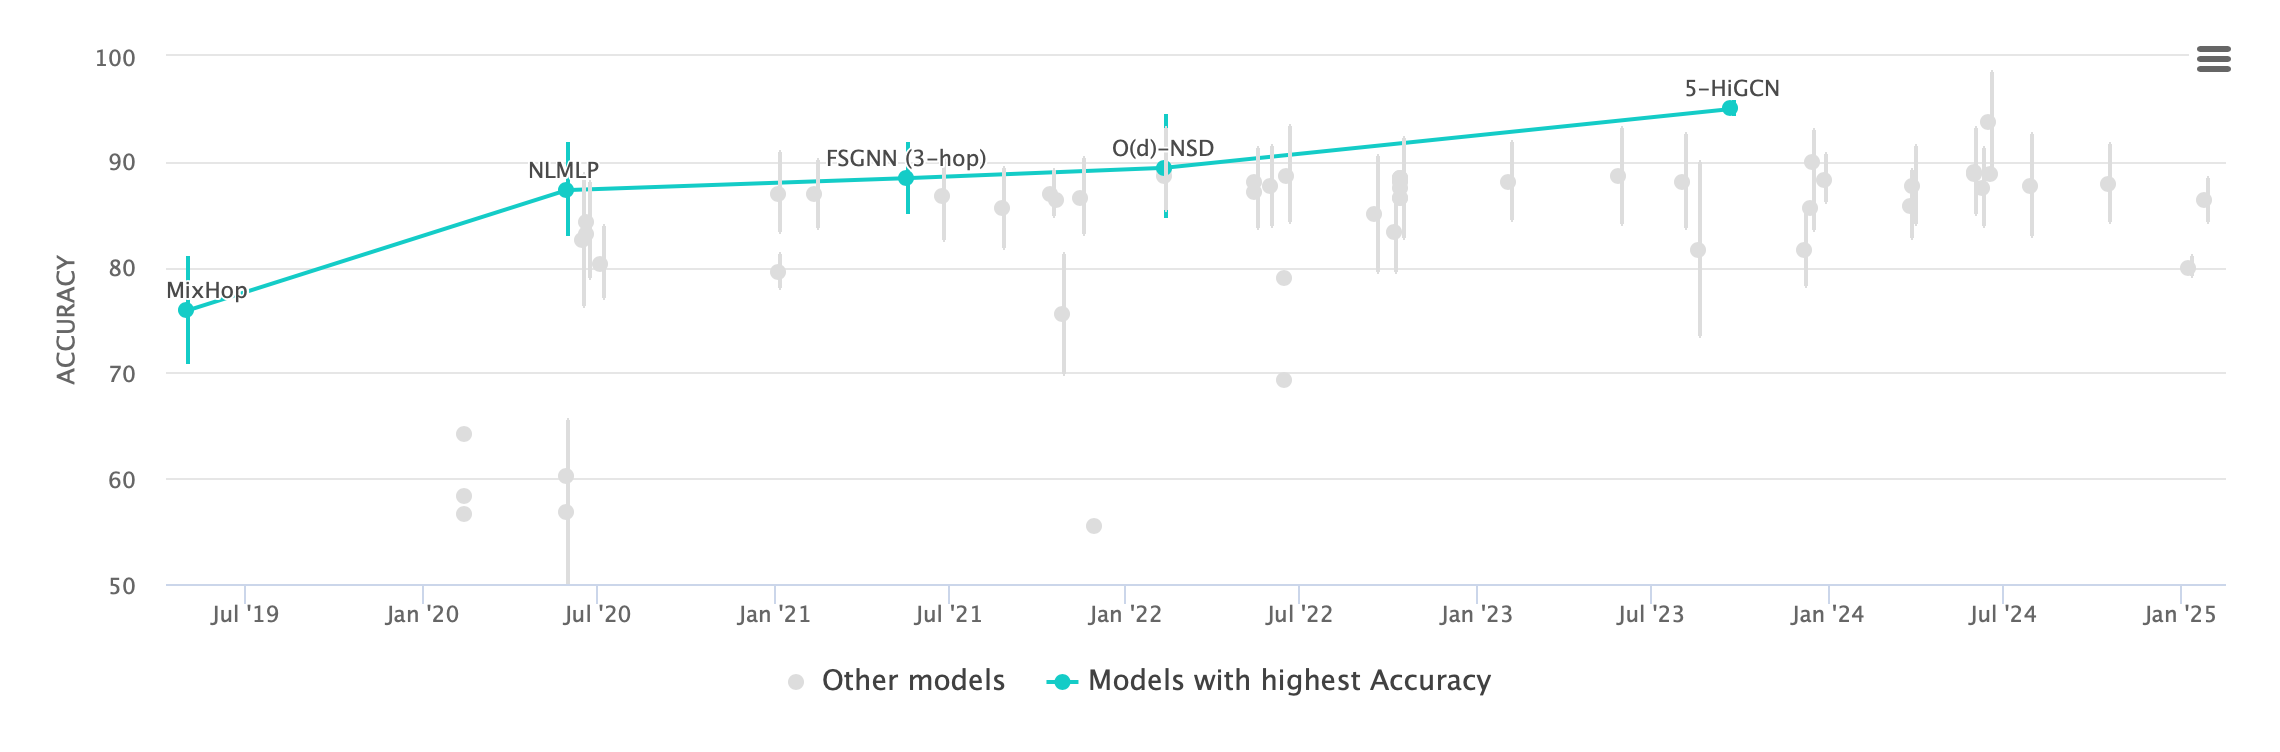
\includegraphics[width=\textwidth]{figures/Wisconsin_leaderboard.png}
    \caption{Performance of GNN on the Wisconsin dataset, from \href{https://paperswithcode.com/sota/node-classification-on-wisconsin}{Paper With Code}.}
    \label{fig:wisconsin_leaderboard}
\end{figure}

The results obtained by \cite{attali2024delaunay} are summarized in the \cref{tab:wisconsin} below.
\begin{table}[h!]
\caption{Experimental results with Delaunay Rewiring in different dimensions reduction for Wisconsin dataset}
\centering
\begin{tabular}{rccccccc}
\hline
\textbf{Metric}            & \textbf{Original} & \textbf{DR (dim=2)} & \textbf{DR (dim=3)} & \textbf{DR (dim=4)} & \textbf{DR (dim=5)} & \textbf{DR (dim=7)} & \textbf{Ours} \\ \hline
Homophily                  & 0.06                   & 0.65                & 0.63                & 0.60                & 0.54                & 0.44             & 0.71   \\ 
Number of edges            & 499                    & 1470                & 2534                & 4064                & 6266                & 16148             & -  \\ 
Max degree                 & 24                     & 14                  & 24                  & 42                  & 57                  & 167               &  14 \\ 
Mean degree                & 12                     & 6                   & 12                  & 18                  & 28                  & 66                & 8  \\ 
Accuracy GCN (\%)          & 55.12 ± 1.51           & \textbf{70.98 ± 1.5}         & 69.45 ± 1.5         & 68.59 ± 1.5         & 68.55 ± 1.5         & 66.42 ± 1.7   & 67.55      \\ 
Accuracy GAT (\%)          & 46.05 ± 1.49           & \textbf{74.33 ± 1.24}        & 74.23 ± 1.4         & 70.75 ± 1.4         & 72.43 ± 1.5         & 67.16 ± 1.7    & 69.12     \\ 
Triangulation time (s) & -                      & $\leq$ 1                 & $\leq$ 1                 & $\leq$ 1           & 2                   & 50               &$\leq$ 1    \\ \hline
\end{tabular}
\label{tab:wisconsin}
\end{table}


%%%%%%%%%%%%%%%%%%%%%%%%%%%%%%%%%%%%%%%%%%%%%%%%%%%%%%%%%%%%%%%%%%%%%%%%%%%%%%%
\subsection{Graph Neural Networks}
We used two popular GNN architectures: Graph Convolutional Networks (GCN) and Graph Attention Networks (GAT).
\begin{table}[h!]
\caption{Hyperparameters for GCN and GAT Models}
\centering
\begin{tabular}{|l|c|c|}
\hline
\textbf{Hyperparameter}       & \textbf{GCN}                          & \textbf{GAT}                          \\ \hline
Hidden Channels               & $32$                                  & $32$                                  \\ \hline
Layers                        & $2$ (ReLU activation)                 & $2$ ($8$ attention heads in $1$st layer, $1$ in $2$nd) \\ \hline
Dropout                       & $0.5$                                 & $0.5$                                 \\ \hline
Learning Rate                 & $0.005$                               & $0.005$                               \\ \hline
Weight Decay                  & $5 \times 10^{-6}$                    & $5 \times 10^{-6}$                    \\ \hline
Training Time per Epoch       & $0.1$s (empirical)                    & $0.2$s (empirical)                    \\ \hline
\end{tabular}
\label{tab:hyperparameters}
\end{table}
%%%%%%%%%%%%%%%%%%%%%%%%%%%%%%%%%%%%%%%%%%%%%%%%%%%%%%%%%%%%%%%%%%%%%%%%%%%%%%%
\subsection{Experimental setup}
\paragraph{Hardware and Software}
The experiments were conducted on a CUDA-enabled GPU with the following software dependencies:
\begin{itemize}
    \item \textbf{Device}: CUDA-enabled GPU with \texttt{PyTorch Geometric, UMAP, NetworkX, GraphRicciCurvature}
    \item \textbf{Preprocessing}: Feature normalization.
    \item \textbf{Runs}: 10 per experiment, max 2000 epochs, early stopping patience 100 epochs.
\end{itemize}

\textbf{Preprocessing Time}:
\begin{itemize} 
    \item UMAP dimensionality reduction: ~1-2 seconds.
    \item Delaunay triangulation: $< 1$ second.
    \item Curvature calculation: $\sim 3-5$ seconds per graph.
    \item Total preprocessing overhead: $\sim 5-8$ seconds.
\end{itemize}

\begin{table}[h!]
\caption{Training Metrics Comparison}
\centering
\begin{tabular}{|l|c|c|c|}
\hline
\textbf{Average Epochs Until Convergence} & \textbf{Baseline} & \textbf{Delaunay} & \textbf{s/epoch}\\ \hline
GCN                          & $\sim 150$ epochs       & $\sim 130$ epochs       & $0.1$s\\ \hline
GAT                          & $\sim 180$ epochs       & $\sim 160$ epochs       & $0.2$s\\ \hline

\end{tabular}
\label{tab:training_metrics}
\end{table}

\paragraph{Memory Usage}
Peak memory during preprocessing: $\sim 2GB$, Training memory footprint: Baseline: $\sim~1GB$;
Delaunay: $\sim 1.2GB$. Additional storage for results: $< 100$MB.

%%%%%%%%%%%%%%%%%%%%%%%%%%%%%%%%%%%%%%%%%%%%%%%%%%%%%%%%%%%%%%%%%%%%%%%%%%%%%%%
\subsection{Results}
Our experiment modestly reaches a 69.12\% accuracy on the Wisconsin dataset,
which has been outperformed by other methods since 2019 has shown in the leaderboard \cref{fig:wisconsin_leaderboard}.
The results are summarized in \cref{tab:graph_comparison}.
\begin{table}[h!]
    \caption{Comparison of Baseline and Delaunay Graph Metrics}
    \centering
    \begin{tabular}{|l|c|c|}
    \hline
    \textbf{Metric}          & \textbf{Orignal} & \textbf{Delaunay Graph} \\ \hline
    Mean Degree              & 5.59                   & 7.85               \\ \hline
    Homophily                & 0.366                  & 0.710 ($\uparrow$ 96\%) \\ \hline
    Curvature Range          & [-0.475, 0.250]        & [-0.214, 0.200]         \\ \hline
    GCN accuracy             & 54.90\%                & 67.55\% ($\uparrow$ 12.6\%)       \\ \hline
    GAT accuracy             & 55.88\%                & 69.12\% ($\uparrow$ 13.2\%)       \\ \hline
    \end{tabular}
    \label{tab:graph_comparison}
    \end{table}


\paragraph{Conclusion}
The Delaunay rewiring approach demonstrates significant and consistent improvements
 on the Wisconsin dataset. The improvements are not only substantial in magnitude 
 $(12.6-13.2\%)$ but also statistically significant, with both GCN and GAT models
 benefiting from the rewiring. The enhanced graph properties (improved homophily 
 and reduced negative curvature) provide structural evidence for why the approach 
 works well. While there are some limitations and areas for future investigation, 
 the current results strongly support the effectiveness of this approach for 
 improving graph neural network performance.

%%%%%%%%%%%%%%%%%%%%%%%%%%%%%%%%%%%%%%%%%%%%%%%%%%%%%%%%%%%%%%%%%%%%%%%%%%%%%%%
% Cayley
%%%%%%%%%%%%%%%%%%%%%%%%%%%%%%%%%%%%%%%%%%%%%%%%%%%%%%%%%%%%%%%%%%%%%%%%%%%%%%%


    
    
%%%%%%%%%%%%%%%%%%%%%%%%%%%%%%%%%%%%%%%%%%%%%%%%%%%%%%%%%%%%%%%%%%%%%%%%%%%%%%%
%%%%%%%%%%%%%%%%%%%%%%%%%%%%%%%%%%%%%%%%%%%%%%%%%%%%%%%%%%%%%%%%%%%%%%%%%%%%%%%


\end{document}


% This document was modified from the file originally made available by
% Pat Langley and Andrea Danyluk for ICML-2K. This version was created
% by Iain Murray in 2018, and modified by Alexandre Bouchard in
% 2019 and 2021 and by Csaba Szepesvari, Gang Niu and Sivan Sabato in 2022.
% Modified again in 2023 and 2024 by Sivan Sabato and Jonathan Scarlett.
% Previous contributors include Dan Roy, Lise Getoor and Tobias
% Scheffer, which was slightly modified from the 2010 version by
% Thorsten Joachims & Johannes Fuernkranz, slightly modified from the
% 2009 version by Kiri Wagstaff and Sam Roweis's 2008 version, which is
% slightly modified from Prasad Tadepalli's 2007 version which is a
% lightly changed version of the previous year's version by Andrew
% Moore, which was in turn edited from those of Kristian Kersting and
% Codrina Lauth. Alex Smola contributed to the algorithmic style files.
